% !TEX root =  master.tex
\chapter{Entwurf}\label{entwurf}
	\section[Design Entwurf]{Design Entwurf {\hfill \normalsize Dennis Köhler}}\label{design}
		
		Damit eine klare Struktur für die Frontend Entwicklung gegeben ist und mehrere Entwickler auf gleichem Wissensstand mit dem Programmieren beginnen können ist ein Entwurf essentiell. Der Design Entwurf stellt die erste konkrete Idee für das Frontend dar und wurde auf Basis der Analyse marktführender Kinowebseiten erstellt. Er soll nicht als strenge Richtlinie für die Umsetzung verstanden werden, sondern ist vielmehr als Orientierungshilfe und Unterstützung zu verstehen. Die wichtigsten Unterschiede zur realisierten Umsetzung werden später im Abschnitt \vref{subdesign} dargestellt. 
		
		Der Entwurf wurde in einem kleineren Team mithilfe diverser Zeichenapps auf dem iPad erstellt. Auch wenn eine Reihe an Tools wie \enquote{Mockingbird} oder \enquote{wireframe.cc} für genau diesen Anwendungsfall gedacht sind, wurde sich bewusst dagegen entschieden. Gründe hierfür sind zum Beispiel die benötigte Einarbeitungszeit in das entsprechende Tool oder deren reduzierter Funktionsumfang in kostenlosen Testversionen. 
		Als Mockup dargestellt wurden die drei Hauptseiten: Startseite, Programm und Sitzplan, welche den Funktionsumfang des Reservierungsprozesses enthalten, abbilden. Die Startseite ist in Abbildung \ref{fig:mockUpStartseite} zu sehen.
		
		\begin{figure}[H]
			\centering 
			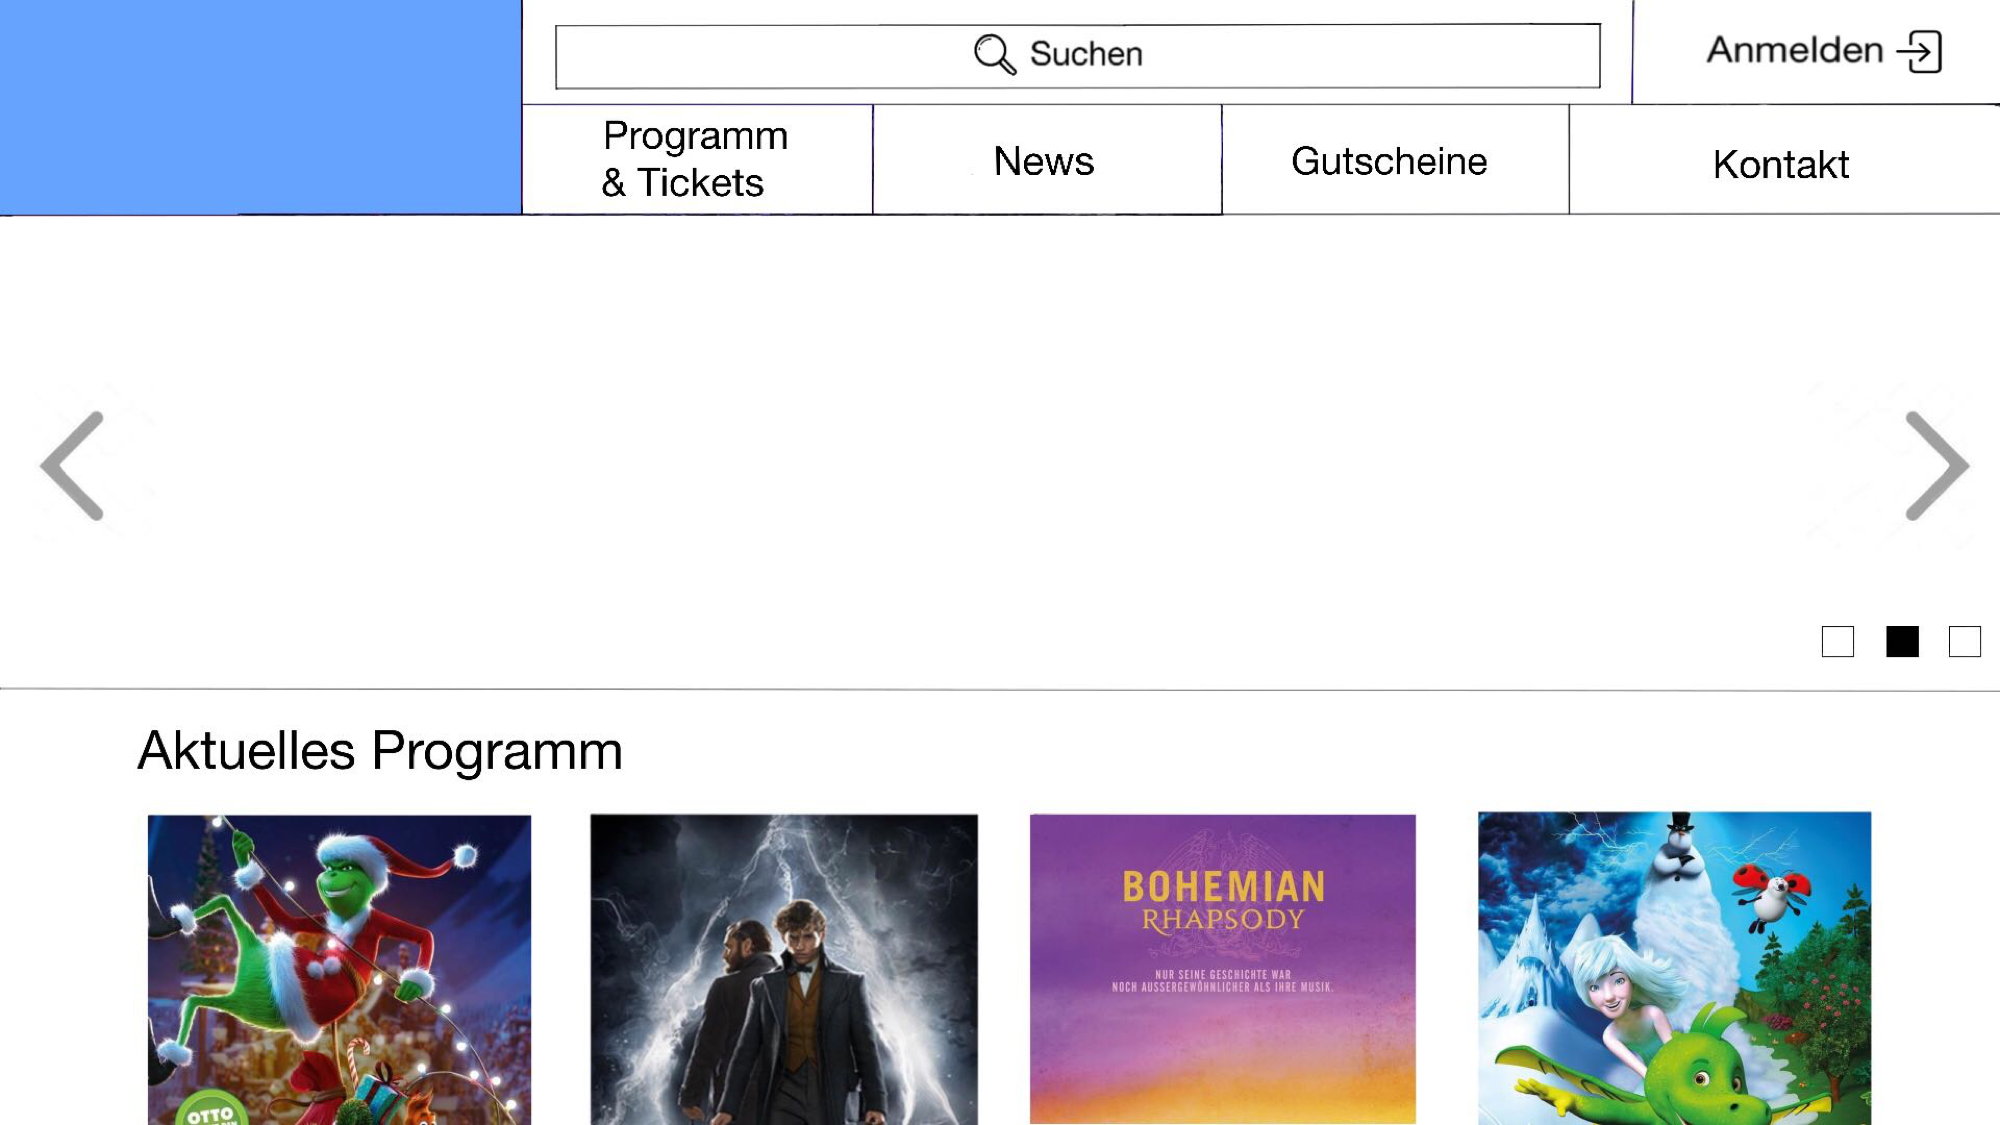
\includegraphics[width=10.8cm]{img/mockUp1.png}
			\captionsetup{format=hang}
			\caption[Mockup Startseite]{\label{fig:mockUpStartseite} Mockup Startseite }
		\end{figure}
		
		Die Navigationsleiste unterscheidet sich zwischen den verschiedenen Seiten nicht. Die blaue Box in der linken, oberen Ecke ist als Platzhalter für das \ac{ICS}-Logo gedacht. Die Navigationsleiste teilt sich in zwei Spalten auf und die einzelnen Sektionen sind eindeutig durch Linien voneinander getrennt. Die Startseite selbst besteht aus einen Slider, welcher möglicherweise aktuelle Filme oder Angebote beinhalten könnte, und dem aktuellen Programm. Dieses wird über die entsprechenden Filmplakate dargestellt, welche einen Link zu fortführenden Informationen implementieren sollen.
		
		\begin{figure}[H]
			\centering 
			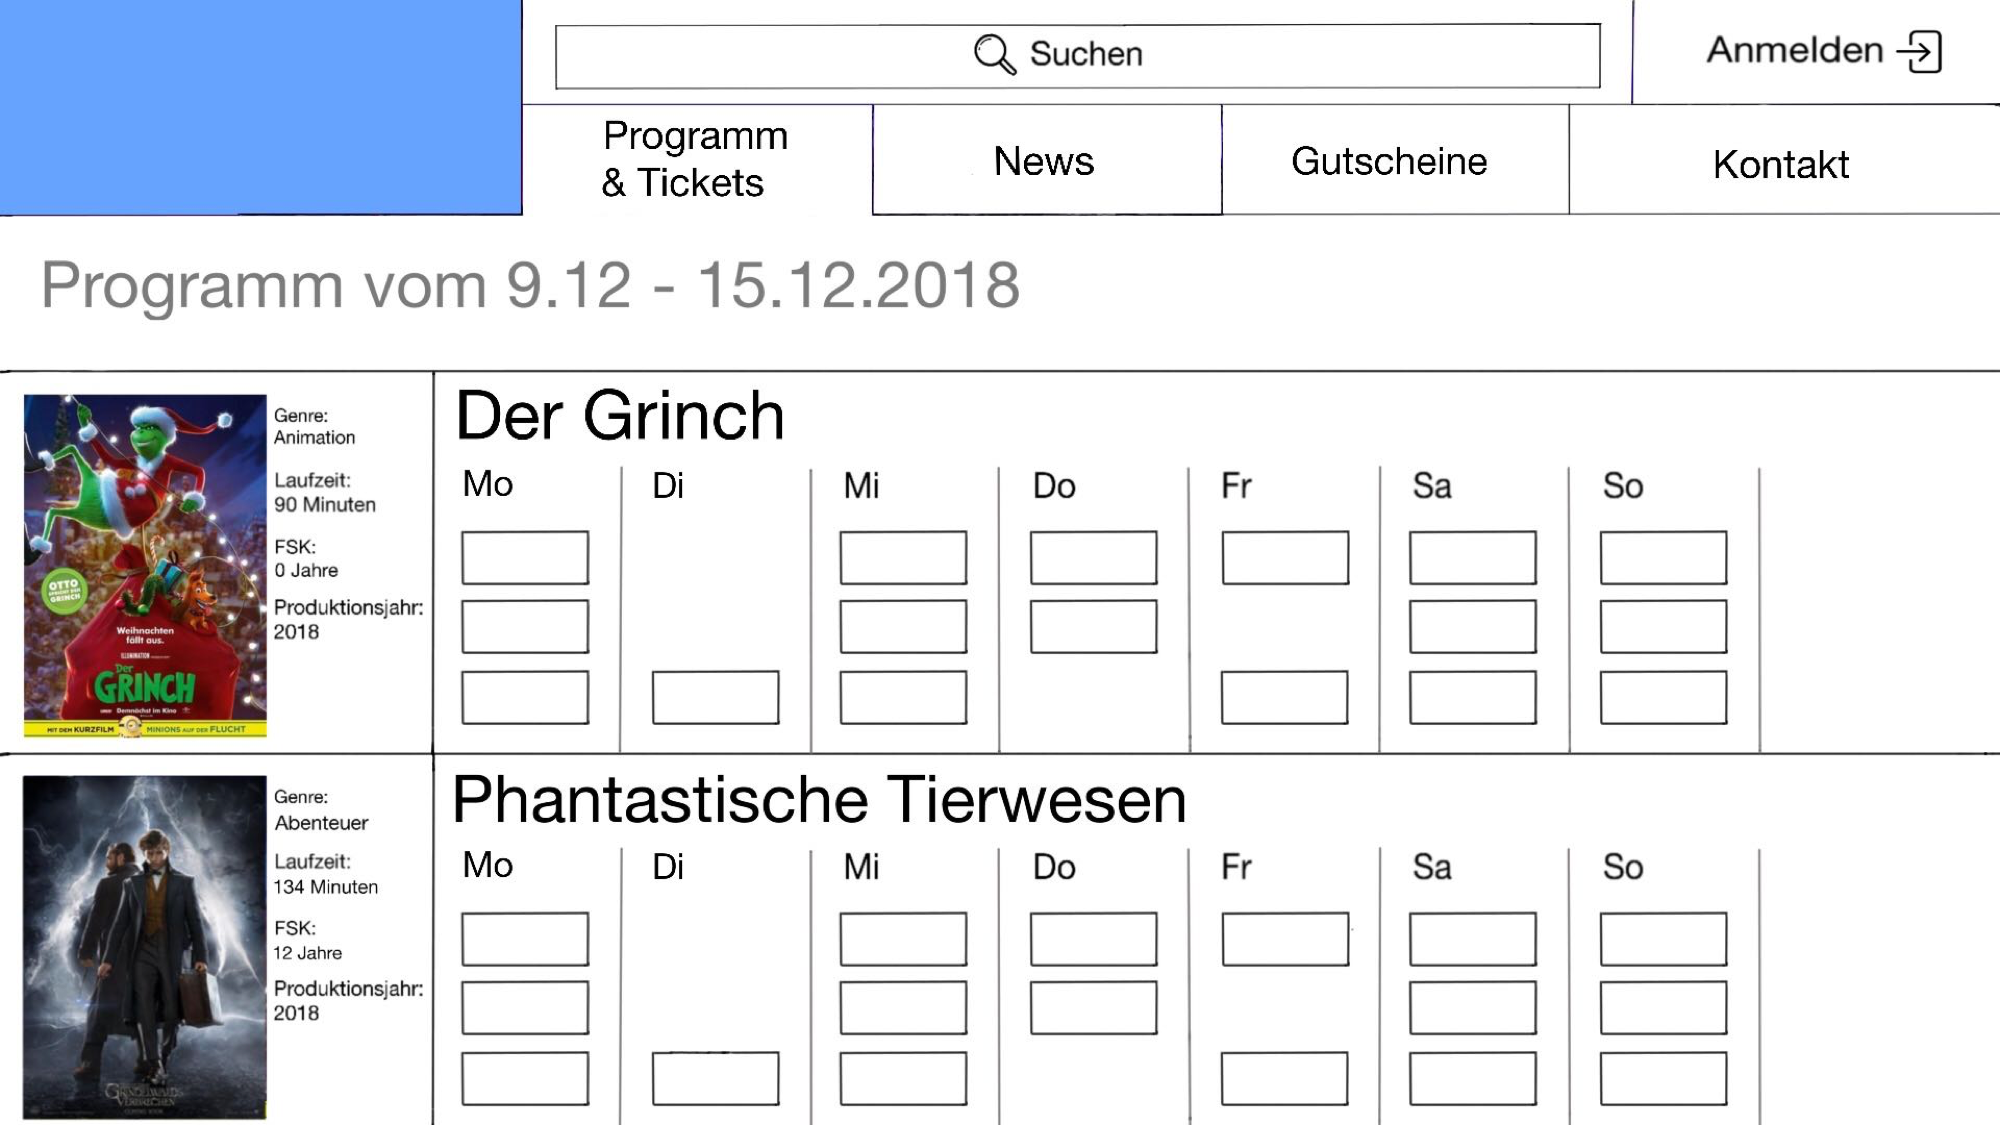
\includegraphics[width=12cm]{img/mockUp2.png}
			\captionsetup{format=hang}
			\caption[Mockup Programm]{\label{fig:mockUpProgramm} Mockup Programm }
		\end{figure}
		
		Die nächste Ansicht zeigt das Programm, also die Filme mit ihren Vorstellungen. Die Filme werden tabellarisch untereinander in Spalten aufgereiht. In jeder Spalte werden auf der linken Seite noch einmal wesentliche Informationen bereitgestellt, während auf der Rechten der Kalenderausschnitt für die jeweilige Woche zu sehen ist. Die Laufzeiten der Filme werden im Mockup als Kästchen symbolisiert, welche später durch entsprechende Uhrzeiten zu ersetzen sind. Diese Kästchen sollen durch einen klick zur nächsten Seite führen: der Detailansicht einer Vorstellung mit Sitzplan.
		
		In Abbildung \ref{fig:mockUpSitzplan} sind noch einmal die Eckdaten der ausgewählten Vorstellung zu sehen. Darunter soll der Nutzer über zwei Eingabefelder die Anzahl, als auch den Typ der gewünschten Plätze auswählen können. Mithilfe des Sitzplans kann nun eine genauere Auswahl der Sitze erfolgen. Die Quadrate, welche die Sitze darstellen sollen, nehmen hierzu passende Farben an und können durch Klicken ausgewählt werden.
		
		\begin{figure}[H]
			\centering 
			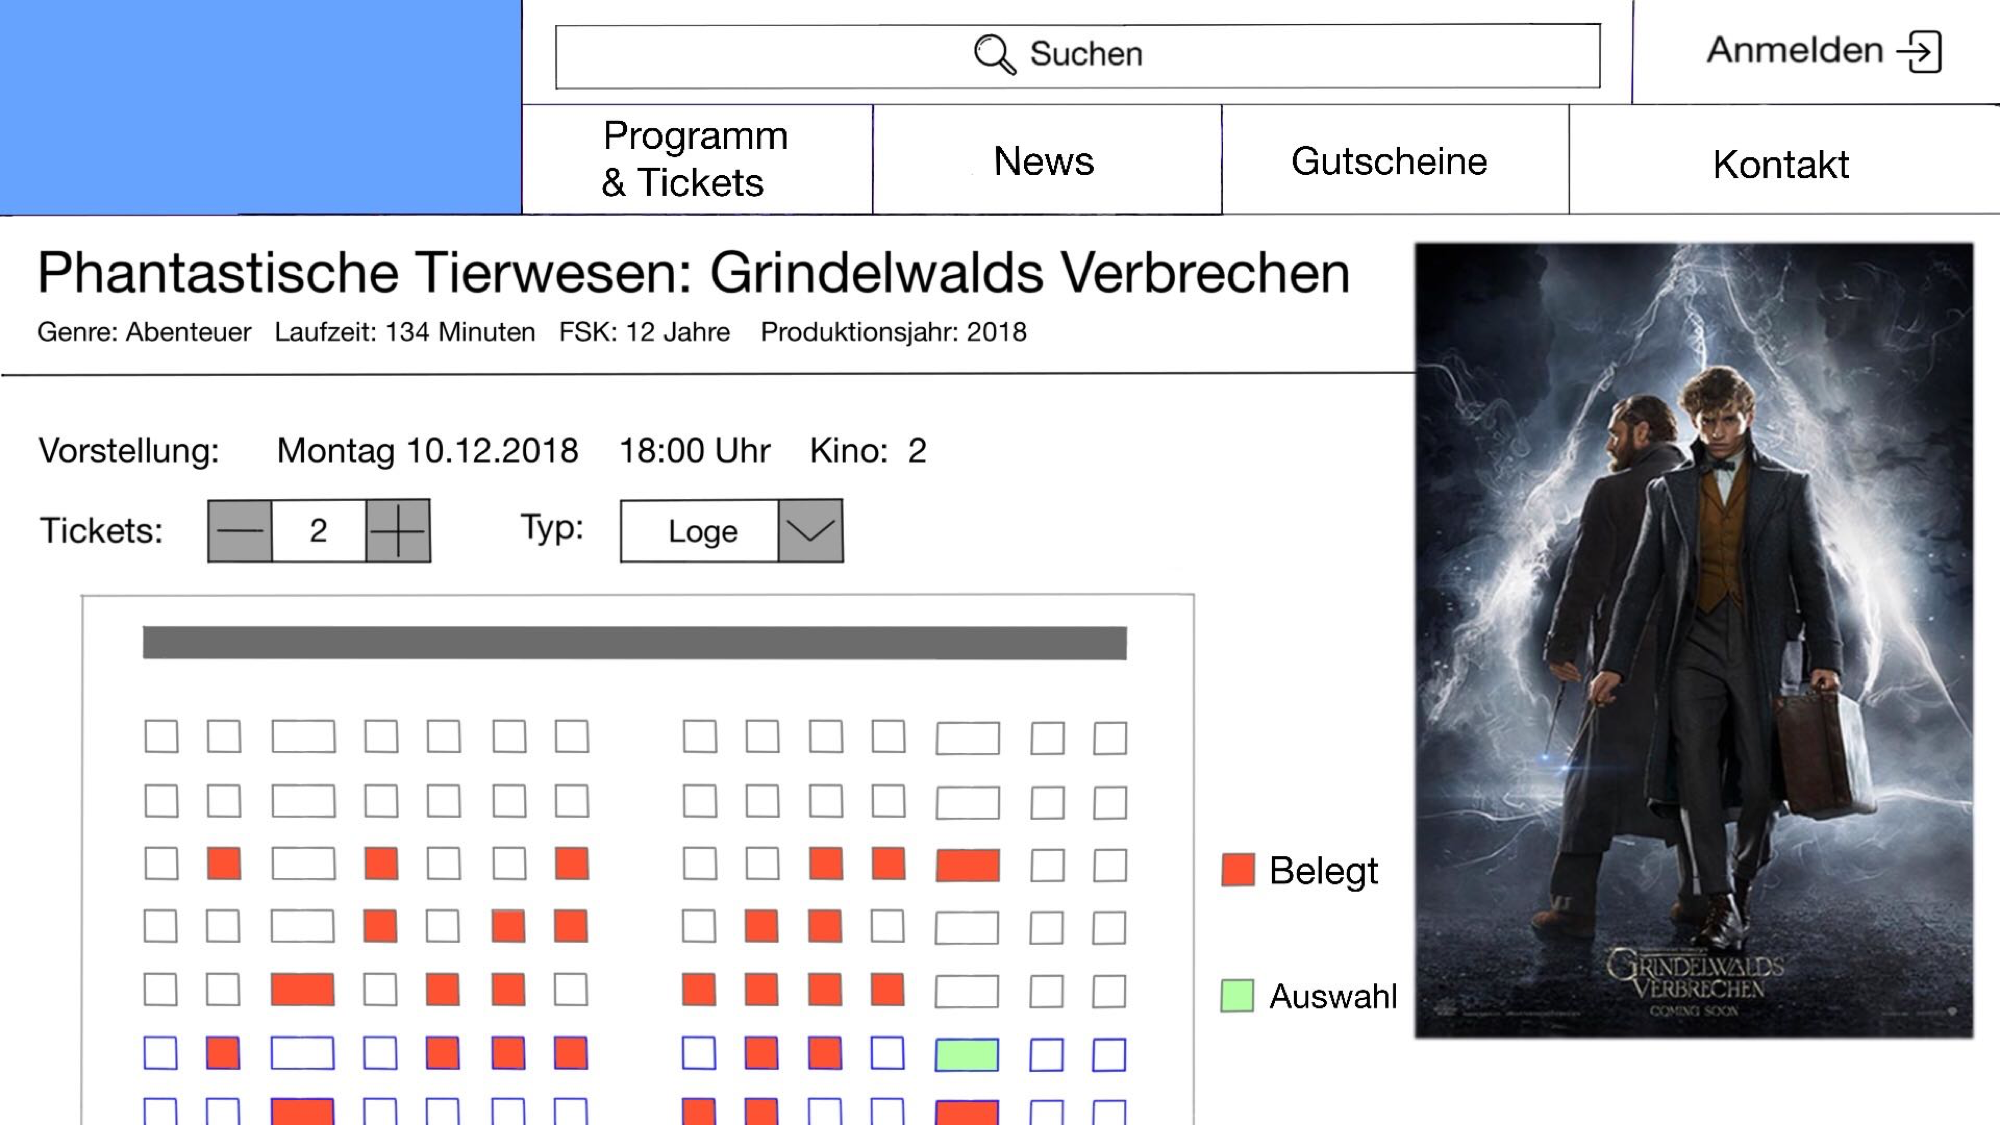
\includegraphics[width=12cm]{img/mockUp3.png}
			\captionsetup{format=hang}
			\caption[Mockup Sitzplan]{\label{fig:mockUpSitzplan} Mockup Sitzplan }
		\end{figure}
		
		
	
	\section[Technischer Entwurf]{Technischer Entwurf{\hfill \normalsize Felix Waage}} 	

		Das \ac{ICS} ist ein komplexes Softwaresystem, welches aus verschiedenen Komponenten, Services und Schichten besteht. Aus diesem Grund war es bereits von Beginn an wichtig, einen genauen Entwurf der späteren Softwarearchitektur zu entwickeln. Diese Vorgehensweise soll vor allem ein möglichst skalierbares, effizientes und anpassungsfähiges Softwaresystem hervorbringen. Des Weiteren wird durch eine gute Dokumentation das System wartungsfreundlicher, da Zusammenhänge schneller erkannt werden können und somit Probleme leichter aufzufinden sind. Auch die Zusammenarbeit der Teammitglieder profitiert von einem ausführlichen technischen Entwurf.
		
			Im weiteren Verlauf dieses Kapitels werden die verschiedenen Schichten erläutert und deren Kommunikation untereinander beschrieben. Darüber hinaus sollen die beteiligten Objekttypen ermittelt und in ein Entitiy-Relationship-Diagramm überführt werden. Das ER-Diagramm dient anschließend als Grundlage für die Entwicklung eines Klassenmodels für das Backend und der Implementierung einer Datenbank für das ICS. 
			
			\subsection{Entwurfsprinzipien}
			Das Ziel der technischen Entwurfsphase ist die Hervorbringung einer skalierbaren, effizienten und anpassungsfähigen Softwarearchitektur. Aus diesem Grund wurden im Vorhinein einige Prinzipien festgelegt, welche bei der Erstellung des technischen Entwurfs beachtet werden sollen, um dieses Ziel zu erreichen.
			%Beim Entwurf eines Softwaresystem ist es besonders wichtig konsistent und gründlich zu arbeiten. Die  Dies ist bedingt durch die Tatsache, dass immer mehrere Personen am \ac{ICS} arbeiten und den Entwurf verstehen müssen.  Aus diesem Grund wurden vor Beginn der Entwicklung des Entwurfs einige Prinzipien festgelegt. Alle Prinzipien, welche folgend aufgelistet und erläutert werden, sollen unter anderem die Übersichtlichkeit, die Wartbarkeit und die Wiederverwendbarkeit des gesamten Projekts oder von Teilen davon ermöglichen.
			\begin{itemize}
				\item \textbf{Das Prinzip einer einzigen Verantwortung} -- Um die Komplexität und Organisation des Softwareprojekts beherrschen zu können, wird das Projekt in verschiedene Module aufgeteilt. Dabei könne einzelene Module wieder aus anderen Modulen zusammen gesetzt sein. Es gilt so Komplexitäten aufzulösen. Jedes Modul übernimmt dabei genau eine Verantwortung und jede Verantwortung wird von genau einem Modul übernommen. Verantwortung ist in diesem Fall die Verpflichtung, eine Anforderung umzusetzen. \autocite[Vgl.][]{Lahres.2015}
				
				\item \textbf{Trennung der Anliegen} -- Jedes Anliegen in einer Anwendung soll durch ein eigenes Modul realisiert werden. Ein mögliches Anliegen wäre zum Beispiel die Transaktionssicherheit, welche unter anderem bei der Reservierung benötigt wird, jedoch auch bei weiteren Anforderung wiederverwendet werden soll.\autocite[Vgl.][]{Lahres.2015} 
				
				\item \textbf{Wiederholungen vermeiden} -- Wenn gleiche Funktionalitäten in einem Softwaresystem mehrfach verwendet werden, sollten diese in ein Modul ausgelagert werden, um mögliche Redundanzen zu vermeiden. Dies könnte vor allem dann zum Problem führen, wenn im Code Fehler entdeckt wurden und dieser Fehler so an mehreren Stellen im Quelltext behoben werden muss. Dies stellt eine große Fehlerquelle dar und sollte somit vermieden werden.\autocite[Vgl.][]{Lahres.2015}
				 
				\item \textbf{Trennung der Schnittstelle von der Implementierung} -- Jedes Modul sollte nur von einer klar definierten Schnittstelle eines anderen Moduls abhängig sein. Dabei spielt die Implementierung der einzelnen Funktionalitäten keine Rolle. Der Quelltext der einzelnen Funktionalitäten soll demnach ausgetauscht werden können, ohne Änderungen an den Schnittstellenaufrufen vornehmen zu müssen. Dies macht das Softwaresystem verständlicher und einfacher zu warten.\autocite[Vgl.][]{Lahres.2015} 
				
				\item \textbf{Testbarkeit} -- Um direkt während der Entwicklung auf Fehler reagieren zu können, ist es wichtig, darauf zu achten, dass sich die einzelnen Module und Softwarekomponenten einzeln testen lassen. So werden neben der eigentlichen Funktionalität auch Unit-Test implementiert. Dies soll möglichst parallel zur Entwicklung der Funktionalität geschehen und muss beim Erstellen des Entwurfs beachtet werden.\autocite[Vgl.][]{Lahres.2015} 
			\end{itemize} 
		
		Wie in vermutlich jedem großen Softwareprojekt kann es zu Sonderfällen kommen, wodurch nicht immer alle Prinzipien genau angewendet wurden. 
		
		\subsection{Schichtenmodell ICS}\label{schichtenmodell}
		
		
		\begin{figure}[H]
			\centering 
			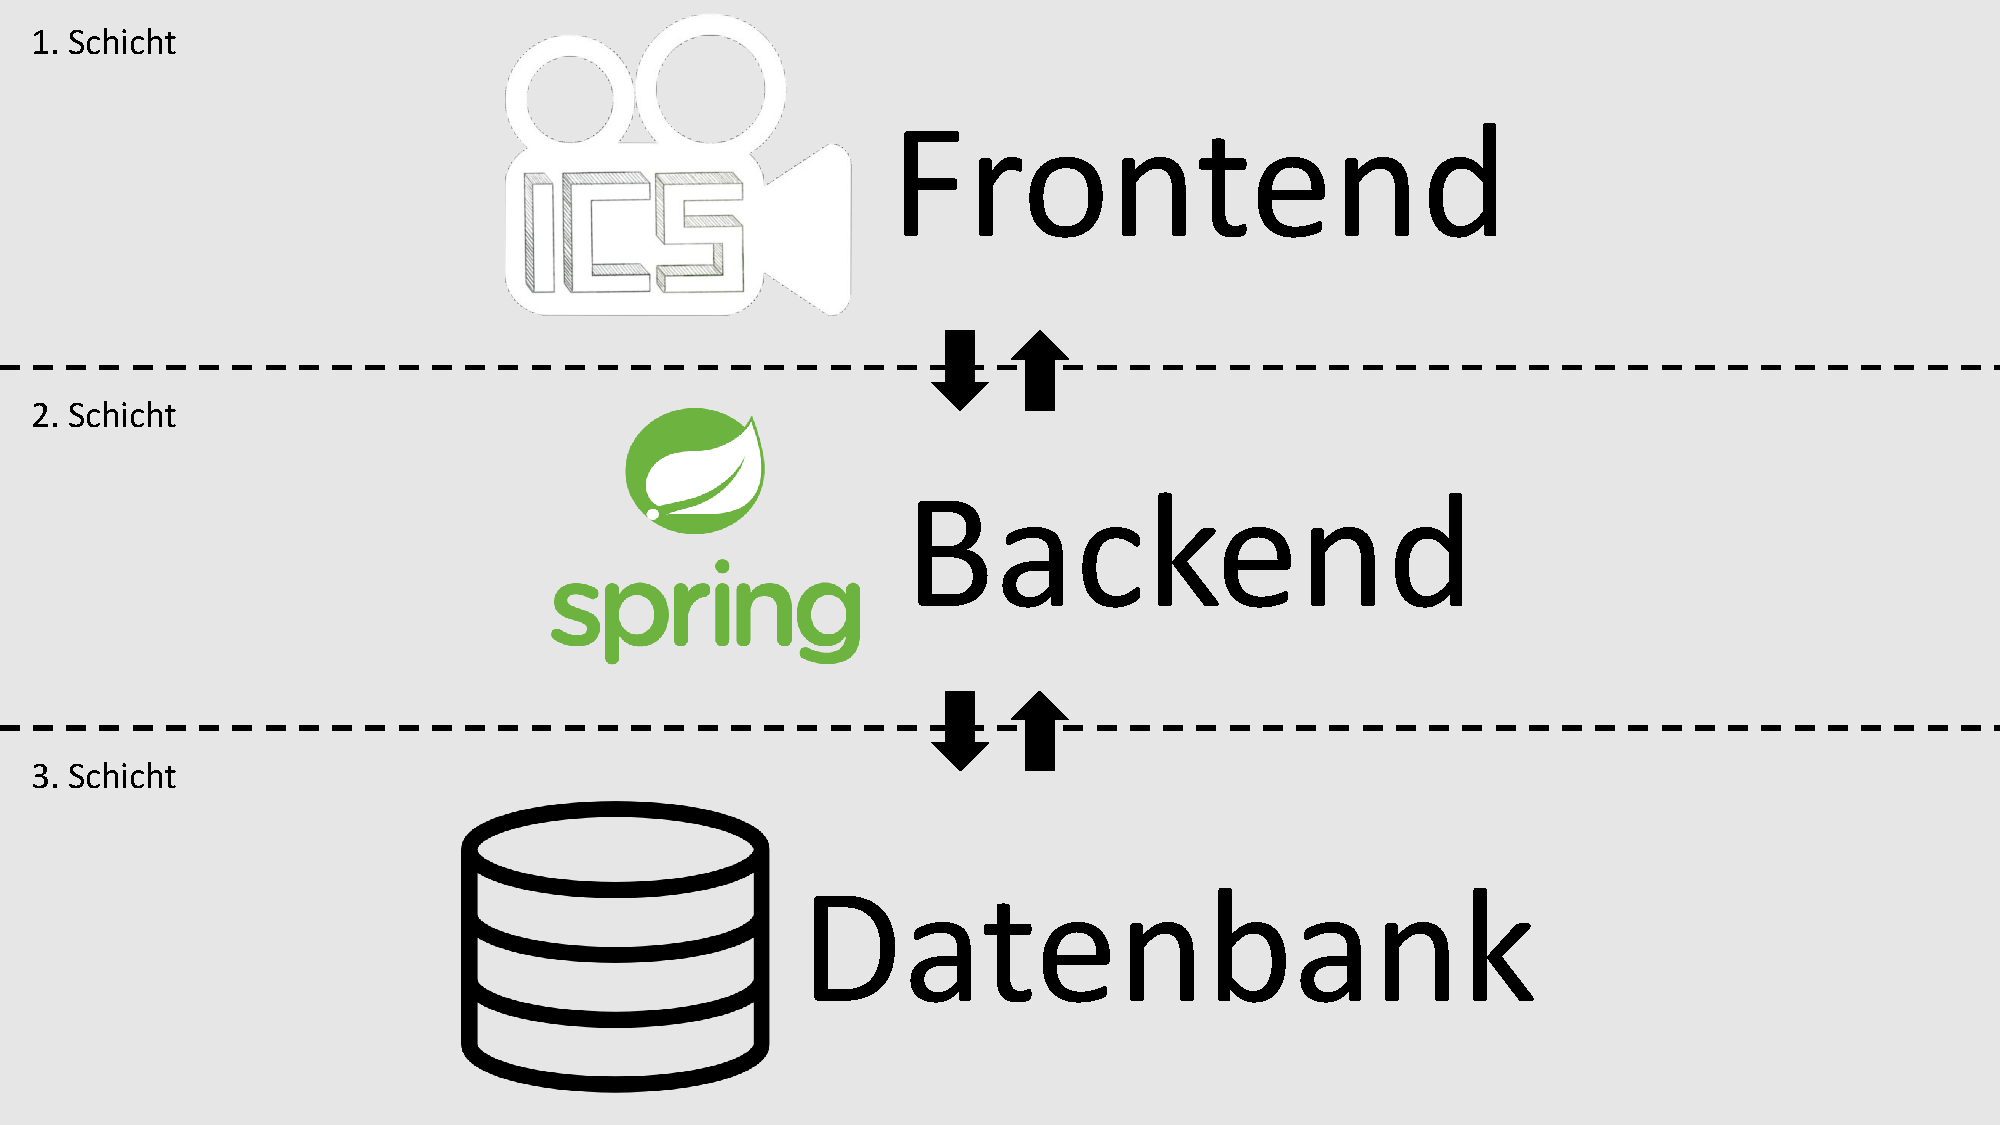
\includegraphics[width=12cm]{img/Schichtenmodell_ICS.pdf}
			\captionsetup{format=hang}
			\caption[Schichtenmodell des ICS]{\label{fig:Schichtenmodell} Schichtenmodell des \ac{ICS} }
		\end{figure}
		
		Die Entwicklung des technischen Entwurfs für das \ac{ICS} wurde damit begonnen, die notwendigen Schichten zu identifizieren und in Relation zueinander zu setzen. Es wurde beschlossen, das Softwaresystem in drei Schichten aufzutrennen. 
		
		Die oberste Schicht ist das \glqq \textbf{Frontend}\grqq{}, welches die grafische Schnittstelle zum Benutzer darstellt. Über das Frontend kann der Benutzer zum Beispiel Filme suchen, Informationen zu Filmen einsehen und Tickets für eine Vorstellung reservieren. Diese Informationen erhält das Frontend durch HTTP-Requests vom Backend.
		
		Im \glqq \textbf{Backend}\grqq{} ist die Fachlogik des Softwaresystem abgebildet, welche zum Beispiel zur Überprüfung der Korrektheit einer Reservierung benötigt wird. Darüber hinaus werden vom Backend die benötigten Rest-Schnittstellen bereitgestellt und die Verbindung zur Datenbank organisiert. 
		
		Die \textbf{Dankbank} dient der Speicherung sämtlicher Daten und Informationen. Sie ist direkt mit dem Backend verbunden und nimmt Anfragen über SQL entgegen. 
		
		Für die Trennung des Softwaresystems in drei Schichten gibt es verschiede Gründe. Zum einen werden für die Implementierung des Frontends andere Technologien verwendet als für das Backend oder die Datenbank. Darüber hinaus verlangen die Anforderungen an das \ac{ICS} eine zentrale Datenhaltung, was sich am besten durch unterschiedliche Schichten realisieren lässt. Darüber hinaus ist durch die Trennung der Schichten eine einfache Skalierung möglich, falls zum Beispiel mehrere Kinos dieses System parallel nutzen möchten.
		\subsection{Entity-Relationship-Modell}\label{chapter:er-diagramm}
		Resultierend aus den Anforderung an das \ac{ICS} gilt es, ein Modell zu entwerfen, welches möglichst genau die spätere Fachlogik repräsentieren kann. Dazu bietet sich für den Anfang das \glqq Entity-Relationship-Modell\grqq{} an.
			
		Das \textit{\glqq Entity-Relationship-Modell\grqq{}} ist ein Datenmodell, welches zur Modellierung von logischen Datenbeziehungen verwendet wird. Der Vorteil in der ER-Modellierung liegt in der einfachen Übertragbarkeit in ein logisches relationales Datenbankmodell, dem \textit{Relationenmodell von Codd}. Ein ER-Diagramm nach der Chen-Notation besteht aus Folgenden Bestandteilen:\autocite[Vgl.][]{Stobitzer.0130201914:40Uhr}
			\begin{itemize}
				\item \textbf{Entität/Entität-Typ} -- Unter einer Entität versteht man ein Objekt der realen Welt (wie z.B.: Avatar, VW Golf, Peter). Gleichartige Entitäten lassen sich anschließend zu einem Entitätstypen zusammenfassen (z.B.: Filme, Autos, Personen).\autocite[Vgl.][]{Stobitzer.0130201914:40Uhr} 
				\item \textbf{Relation} -- Durch die Relation wird die Beziehung zwischen zwei Entitäten beschrieben. So existiert zum Beispiel eine Beziehung zwischen dem Ticket und einer Person. Darüber hinaus ist die Beziehung zwischen zwei oder mehreren Entitäten durch die Kardinalität näher bestimmt. So kann eine Person mehrere Tickets gekauft haben, wobei ein Ticket nur zu einer Person gehört.\autocite[Vgl.][]{Stobitzer.0130201914:40Uhr}
				\item \textbf{Attribut} -- Attribute beschreiben Entitäten näher und enthalten Informationen wie: Name, Alter, Preis.
			\end{itemize}
		
		Die zuvor erwähnte Chen-Notation wird grafisch folgendermaßen grafisch dargestellt (siehe Abbildung \ref{fig:chennotation}).
					\begin{figure}[H]
						\centering 
						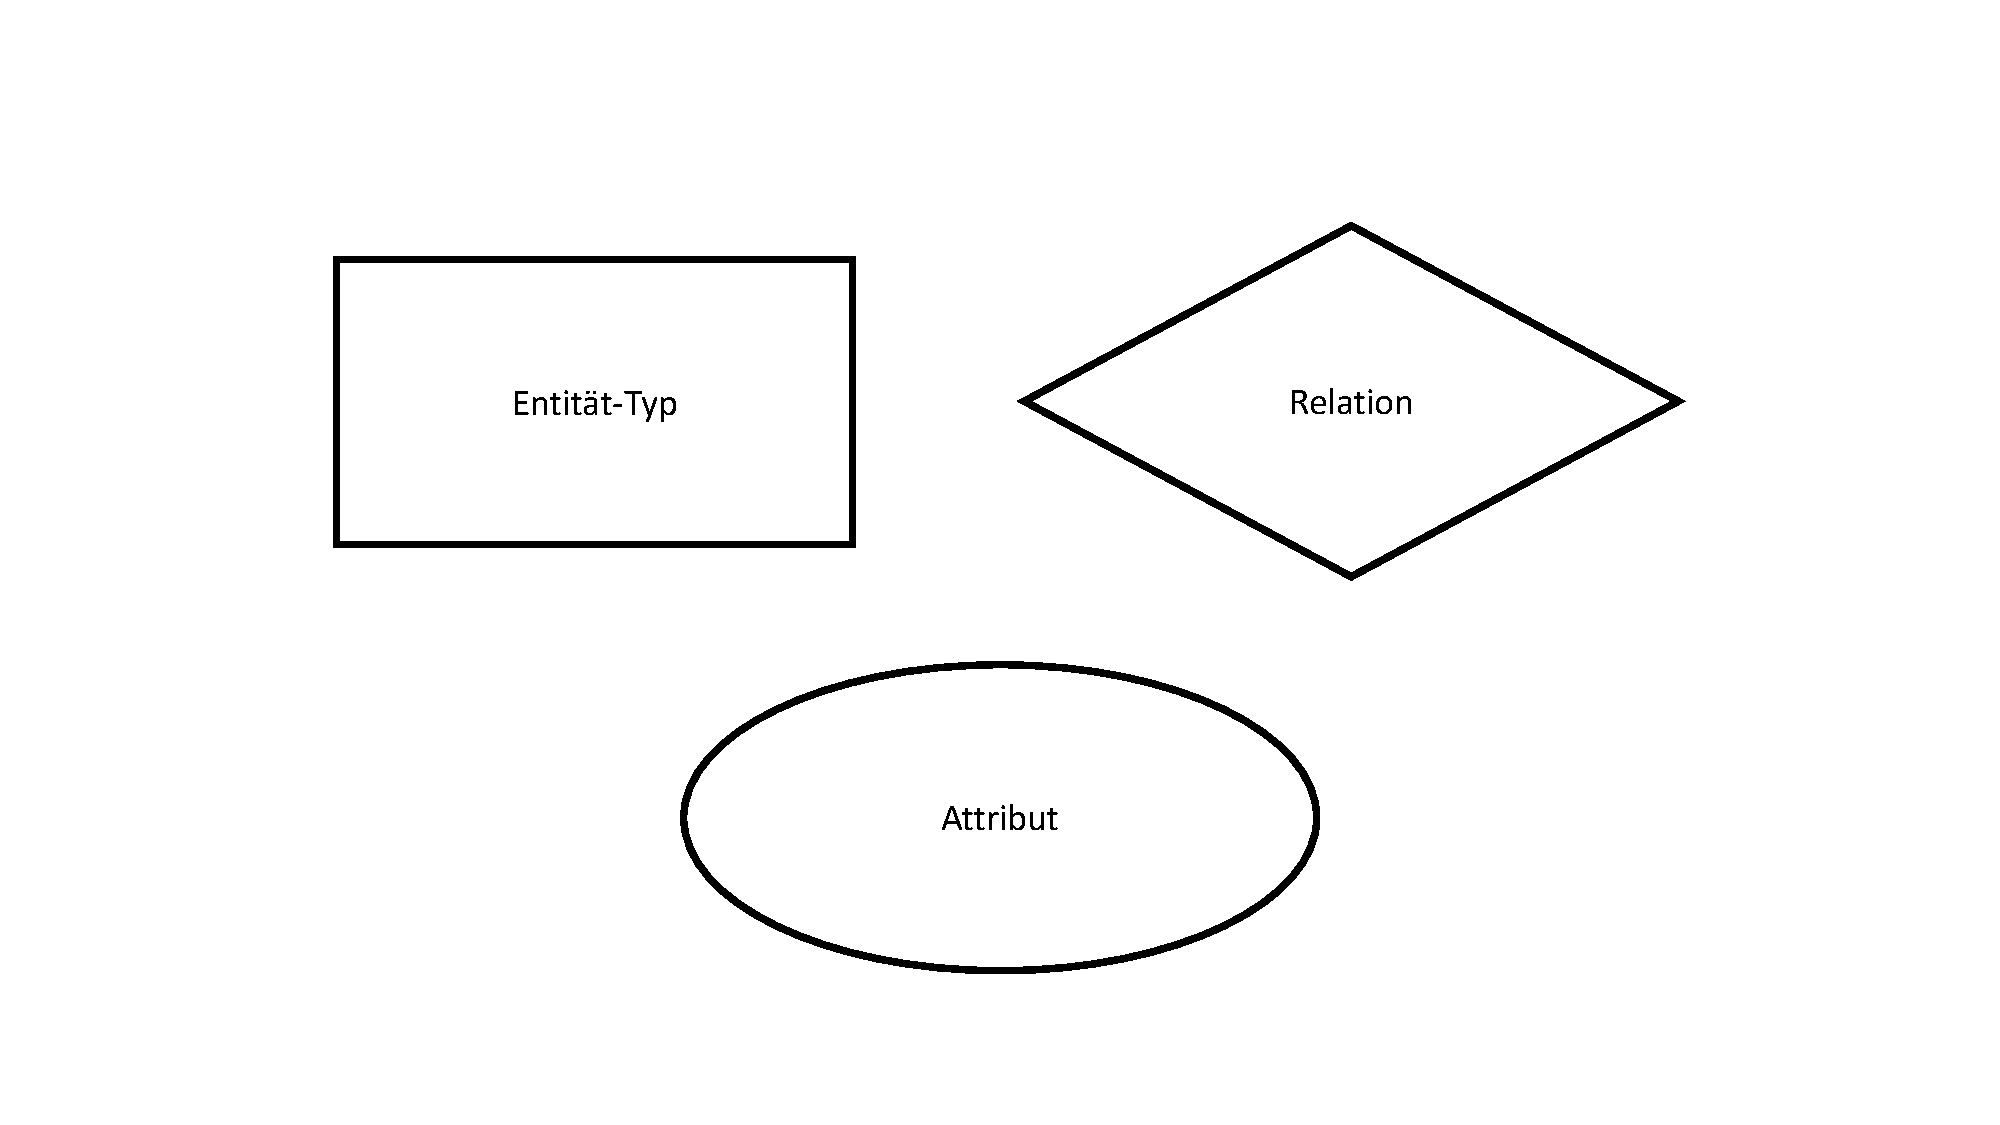
\includegraphics[scale=0.3]{img/ChenNotationERDiagramm.pdf}
						\captionsetup{format=hang}
						\caption[ER-Diagramm Chen-Notation]{\label{fig:chennotation} ER-Diagramm nach der Chen-Notation }
					\end{figure}
		
		Das ER-Diagramm wird auf Grundlage der Ergebnisse der Analysephase erstellt. Dazu werden zu Beginn die beteiligten Entitäten ermitteln. Dies kann besonders gut an der Reservierung eines Tickets erläutert werden. So sind am Reservierungsprozess die Entitäten \textit{Reservierung, Ticket und Benutzer} beteiligt. Im nächsten Schritt werden die Relationen zwischen den Entitäten aufgestellt. Dies kann verbal wie folgt beschrieben werden: Eine Reservierung umfasst immer mindestens ein Ticket. Eine Reservierung wird durch genau einen Benutzer vorgenommen. Aus dieser verbalen Beschreibung der Relationen lassen sich auch die Kardinalitäten bestimmen:
		\begin{itemize}
			\item \textbf{Reservierung \textit{umfasst} Tickets} -- Hier handelt es sich um eine 1:n (n > 0) Beziehung, denn eine Reservierung kann ein oder mehrere Tickets \textit{umfassen}, wobei ein Ticket immer nur zu einer Reservierung gehören kann.
			
			\item  \textbf{Benutzer \textit{macht} Reservierung} -- Eine Reservierung wird immer durch genau einen Benutzer vorgenommen, jedoch kann ein Benutzer mehrere Tickets Reservieren, muss es jedoch nicht, weshalb es sich hier auch um eine 1:n Beziehung handelt, wobei in diesem Fall n auch den Wert 0 annehmen kann. 
		\end{itemize}
		Im letzten Schritt gilt es, die Attribute der einzelnen Entitäten zu ermitteln und in das ER-Diagramm einzutragen. So hat ein Benutzer eine Email-Adresse (\texttt{email}), einen Namen (\texttt{name}) und eine Benutzernummer (\texttt{benutzer\_nr}). Eine Reservierung besitzt eine Reservierungsnummer (\texttt{res\_nr}), ein Datum (\texttt{datum}) und eine Benutzernummer (\texttt{benutzer\_nr}). Und jedes Ticket eine Reservierungsnummer (\texttt{res\_nr}) und eine Ticketnummer (\texttt{ticket\_nr}). Ein Ticket beinhaltet natürlich noch Informationen zur Vorstellung, dem Sitz und dem Preis, jedoch sollen diese zur Vereinfachnung nicht betrachtet werden. Nachfolgend ist das eben erläuterte ER-Diagramm abgebildet (Abbildung \ref{fig:erdiagramm_reservation}).
		
		\begin{figure}[H]
			\centering 
			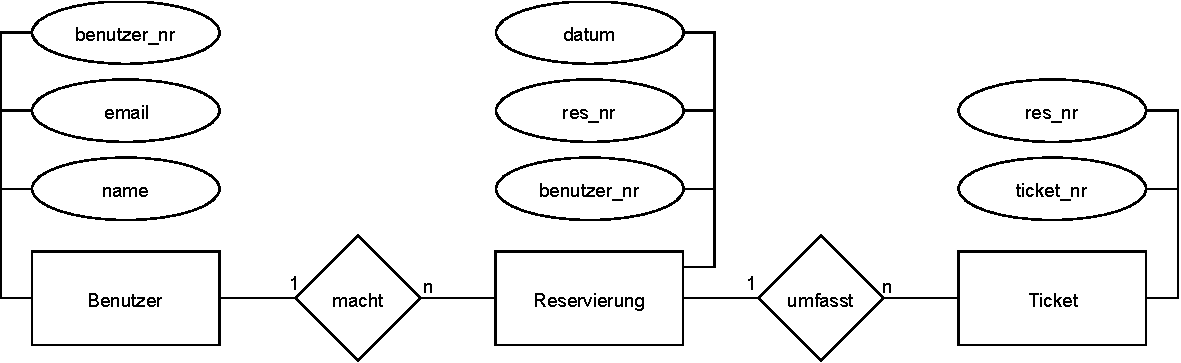
\includegraphics[width=13cm]{img/erdiagramm_reservation.pdf}
			\captionsetup{format=hang}
			\caption[ER-Datenmodell Reservierungsprozess]{\label{fig:erdiagramm_reservation} Entity-Relationship-Diagramm für den Reservierungsprozess}
		\end{figure}
		
		Um die gesamte Funktionalität abbilden zu können, welche in der Analysephase ermittelt wurde, sind weitere Entitäten notwendig. So gehört, wie bereits erwähnt, zu einem Ticket auch eine \texttt{Vorstellung} und eine Vorstellung kann mit	 mehreren Tickets besucht werden. Des Weiteren wird dem Ticket auch ein \texttt{Sitz} zugeordnet und dieser Sitzt befindet sich in einem \texttt{Saal} und ist durch eine \texttt{Sitzkategorie} näher definiert. Einer Vorstellung ist immer genau ein \texttt{Film} zugeordnet, jedoch kann ein Film in mehreren Vorstellungen laufen. Um den Film besser einordnen zu können, steht dieser in Beziehung mit dem \texttt{Genre}. Einem Film kann dabei genau ein Genre zugewiesen werden, wobei mehrere Filme das gleiche Genre besitzen können. Die Preise für ein Ticket ergeben sich aus der \texttt{Sitz-} und \texttt{Vorstellungskategorie}, indem diese jeweils in einer Beziehung zur \texttt{Preiskategorie} stehen. 
		Unter Berücksichtigung der Entitäten und wie diese in Beziehungen zueinander stehen ergibt sich das ER-Diagramm für das \ac{ICS} (Abbildung  \ref{fig:erModell}).
		
		Mit Hilfe des Entity-Relationship-Modell kann nun die Datenbank angelegt werden. Dazu sind bestimmte Regeln und Vorgehensweisen anzuwenden, um die benötigten Tabellen und Spalten aus dem ER-Modell zu extrahieren:
				
		Die Tabellen der Datenbank entsprechen den Entitäten im ER-Modell. Die Attribute werden als Spalten überwiegend unverändert übernommen. Als Schlüssel bietet es sich an, ein zusätzliches Schlüsselattribut zu verwenden, das eine fortlaufende Nummer oder eine \ac{UUID}. Um die Beziehungen zwischen den Attributen richtig abbilden zu können, müssen die Kardinalitäten beachtet werden. 
				\begin{itemize}
					\item 1:1 Beziehung -- Bei dieser Form der Kardinalität enthält eine der beiden Tabellen den Primärschlüssel der anderen Tabelle in Form eines Fremdschlüssels.
					\item 1:n Beziehung -- Liegt diese Form der Kardinalität vor, wird der Primärschlüssel der Entität, die nur einfach in der Beziehung beteiligt ist, als Fremdschlüssel auf der n-Seite hinzugefügt. 
					\item n:m Beziehung -- Sind beide Entitäten in der Beziehung mehrfach beteiligt, gilt es, eine zusätzliche Tabelle anzulegen. Diese enthält die Primärschlüssel der beteiligten Entitäten als Fremdschlüssel.
				\end{itemize}
		
					\begin{figure}[H]
						\centering 
						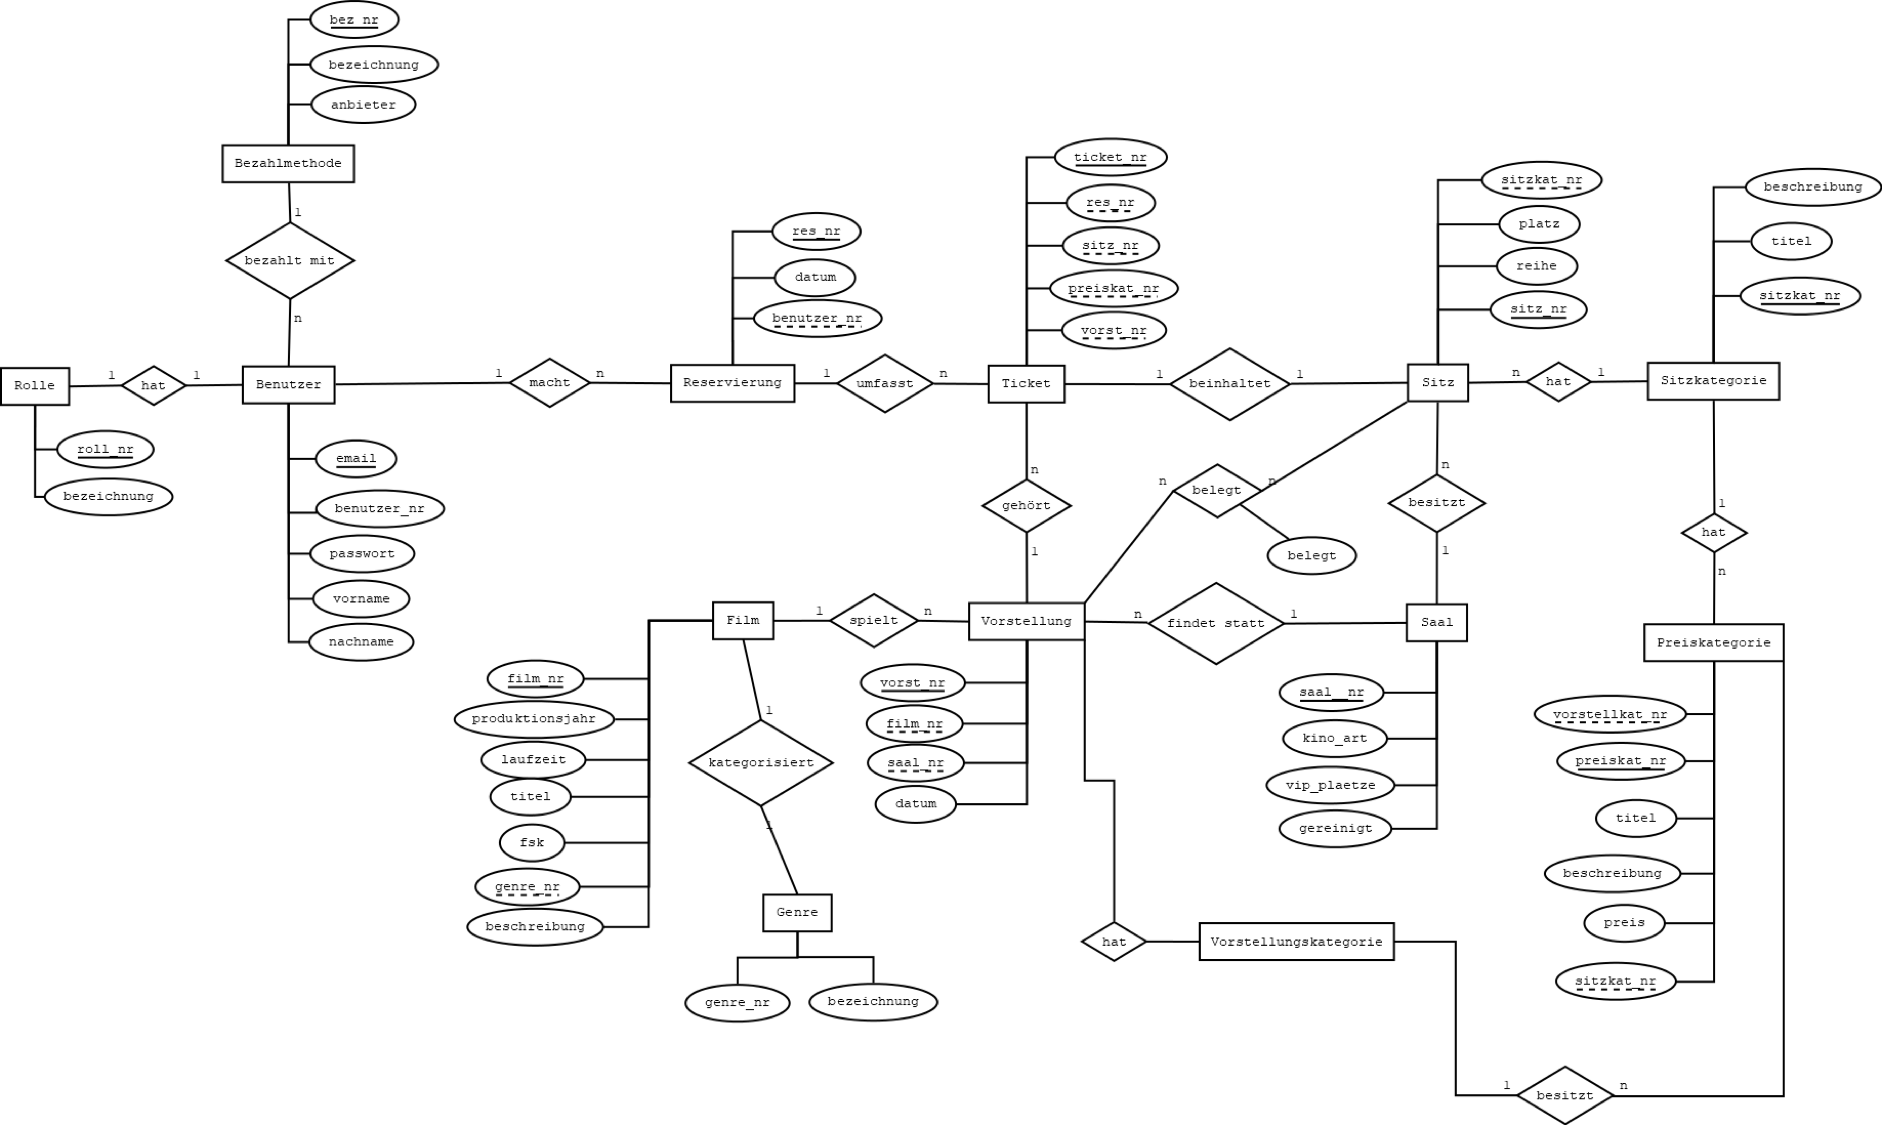
\includegraphics[angle=+90,width=13cm]{img/erModell.png}
						\captionsetup{format=hang}
						\caption[ER-Datenmodell]{\label{fig:erModell} Entity-Relationship-Datenmodell}
					\end{figure}
				
		
		Für das Beispiel des Reservierungsprozesses werden die folgenden Tabellen erstellt: \texttt{Benutzer, Ticket, Reservierung}. Der Benutzer ist an der Beziehung zur Reservierung einfach beteiligt, was dazu führt, dass die Tabelle Reservierung den Primärschlüssel des Benutzers als Fremdschlüssel aufnimmt. Anders verhält es sich bei der Relation zwischen Ticket und Reservierung, denn hier ist die Reservierung einfach beteiligt, wodurch das Ticket den Primärschlüssel als Fremdschlüssel mit speichert. Für dieses Beispiel ergeben sich demnach folgende Datenbanktabellen (Abbildung \ref{fig:database_example}):
		 
		\begin{figure}[H]
			\centering 
			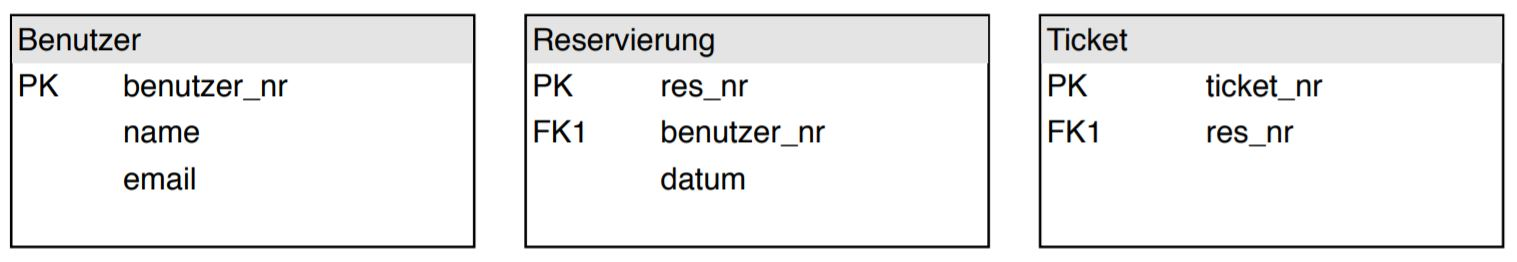
\includegraphics[width=15cm]{img/database_example.JPG}
			\captionsetup{format=hang}
			\caption[Datenbanktabellen Reservierungsprozess]{\label{fig:database_example}Datenbanktabellen für den Reservierungsprozess}
		\end{figure}
		
		\subsection{Klassendiagramm}
		Ein Klassendiagramm dient der strukturierten Darstellung der zu verwendenden Klassen, Schnittstellen sowie deren Beziehungen. Das Klassendiagramm ist die Grundlage für die Implementierung des Backends für das \ac{ICS}, da hier Repräsentanten der Entitäten aus Abschnitt \ref{chapter:er-diagramm} in Form von Java-Objekten benötigt werden, um diese später in der Datenbank speichern zu können. Der Entwurf des Klassendiagramms wurde anhand des zuvor erstellten ER-Diagramms angefertigt. Dabei wurde darauf geachtet, dass die UML-Notation eingehalten wird.
		
		Eine Klasse repräsentiert eine Gruppe von Objekten mit ähnlichen Eigenschaften. Sie besitzt dazu Funktionen und Attribute, welche die Eigenschaften des jeweiligen Objekts definieren. Die einfachste Form einer Klasse ist die anonyme Klasse. Sie wird in UML wie folgt dargestellt (Abbildung \ref{fig:uml_anonym_class}):
		\begin{figure}[H]
			\centering 
			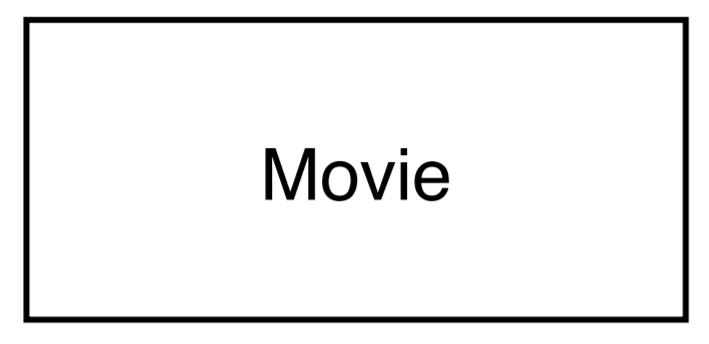
\includegraphics[width=4cm]{img/uml_anonym_class.JPG}
			\captionsetup{format=hang}
			\caption[Anonyme Klasse in UML-Notation]{\label{fig:uml_anonym_class}Anonyme Klasse in UML-Notation}
		\end{figure}
		Diese Darstellung kann durch Attribute und Funktionen erweitert werden, wobei die Sichtbarkeit der Attribute und Funktionen bereits im Klassendiagramm beschrieben werden sollte. In Java sind drei Zugriffsmodifikatoren definiert:
		\begin{itemize}
			\item\textbf{public} -- Es kann von Außen auf das Attribut oder die Funktion direkt zugegriffen werden. Dies kann dazu führen, dass Klassenbestandteile nicht sinngemäß verwendet werden. In UML wird dieser Zugriffsmodifikator durch ein + vor dem Attribut oder der Funktion dargestellt. 
			\item\textbf{private} -- Nur Funktionen innerhalb der Klasse können auf diese Attribute oder Funktionen zugreifen. Die Notation UML beschreibt dies mit einem - vor dem Attribut oder der Funktion.
			\item\textbf{protected} -- Durch den Zugriffmodifikator protected ist es auch Subklassen möglich, auf Attribute und Funktionen zuzugreifen. In der UML-Notation wird dieser Zugriffsmodifikator durch \# repräsentiert.
		\end{itemize}
		Allgemein ist es jedoch üblich, Attribute grundsätzlich als \texttt{private} zu deklarieren und den Zugriff durch sogenannte \textit{Getter- und Setter-Methoden} zu ermöglichen. Dies ermöglicht es, Werte vor dem Speichern auf Korrektheit zu prüfen. Außerdem kann so ein Missbrauch der Klasse für andere Zwecke verhindert werden. Eine Klasse mit all den erwähnten Bestandteilen wird in UML wie folgt dargestellt (Abbildung \ref{fig:KlasseUML}): 
		\begin{figure}[H]
			\centering 
			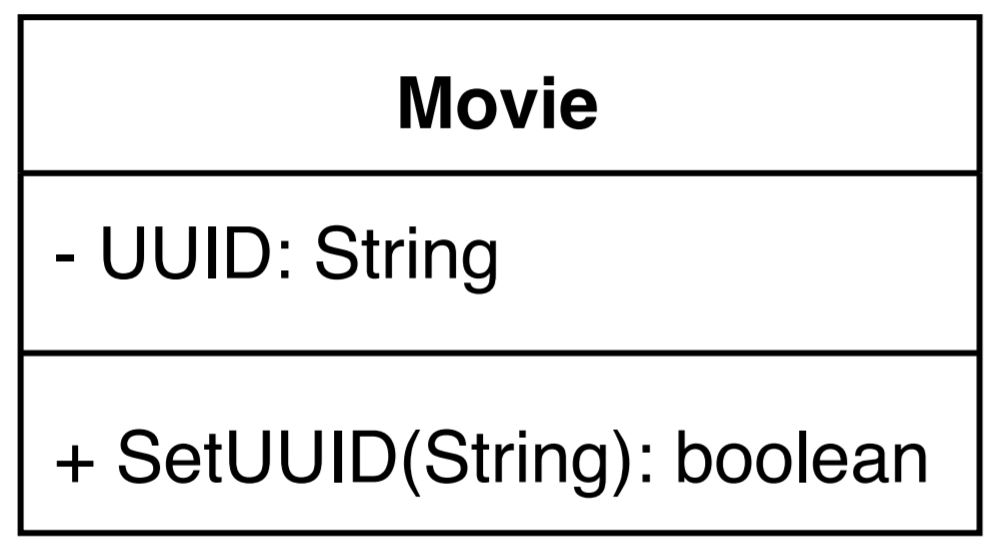
\includegraphics[width=4cm]{img/uml_class.JPG}
			\captionsetup{format=hang}
			\caption[Klasse in UML-Notation]{\label{fig:KlasseUML}Klasse nach der UML-Notation}
		\end{figure}
		Die Relationen zwischen den Klassen werden durch Pfeile und Linien visualisiert, welche wie beim ER-Diagramm an den Enden die Kardinalität der Beziehung angeben. 
		
		\begin{figure}[H]
			\centering 
			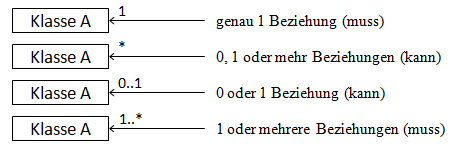
\includegraphics[width=12cm]{img/UmlKardinalitaet.png}
			\captionsetup{format=hang}
			\centering\caption[Kardinalitäten nach UML-Notation]{\label{fig:Kardinalitaeten.UML}Startseite von Kinopolis\footnotemark}
		\end{figure}\footnotetext{Quelle: http://www.info-wsf.de/index.php/Assoziationen\_und\_Kardinalit\%C3\%A4ten}
		
		Neben den Kardinalitäten werden auch Aggregationen und Kompositionen in der UML-Darstellung ermöglicht. Eine \textit{Aggregation} ist eine besondere Form der Beziehung zwischen zwei Klassen. Sie drückt aus, dass eine Klasse Objekte der anderen Klasse als Attribut beinhaltet. Verbal wird dies oft mit \textit{besteht aus, hat, ist Bestandteil von} ausgedrückt. Eine Komposition ist ähnlich zur Aggregation mit dem Unterschied, dass die Existenz der einen Klasse von der Existenz der anderen abhängt. So kann zum Beispiel ein Raum nicht ohne ein Gebäude existieren. In UML wird dies wie folgt dargestellt:
		
		\begin{figure}[H]
			\centering 
			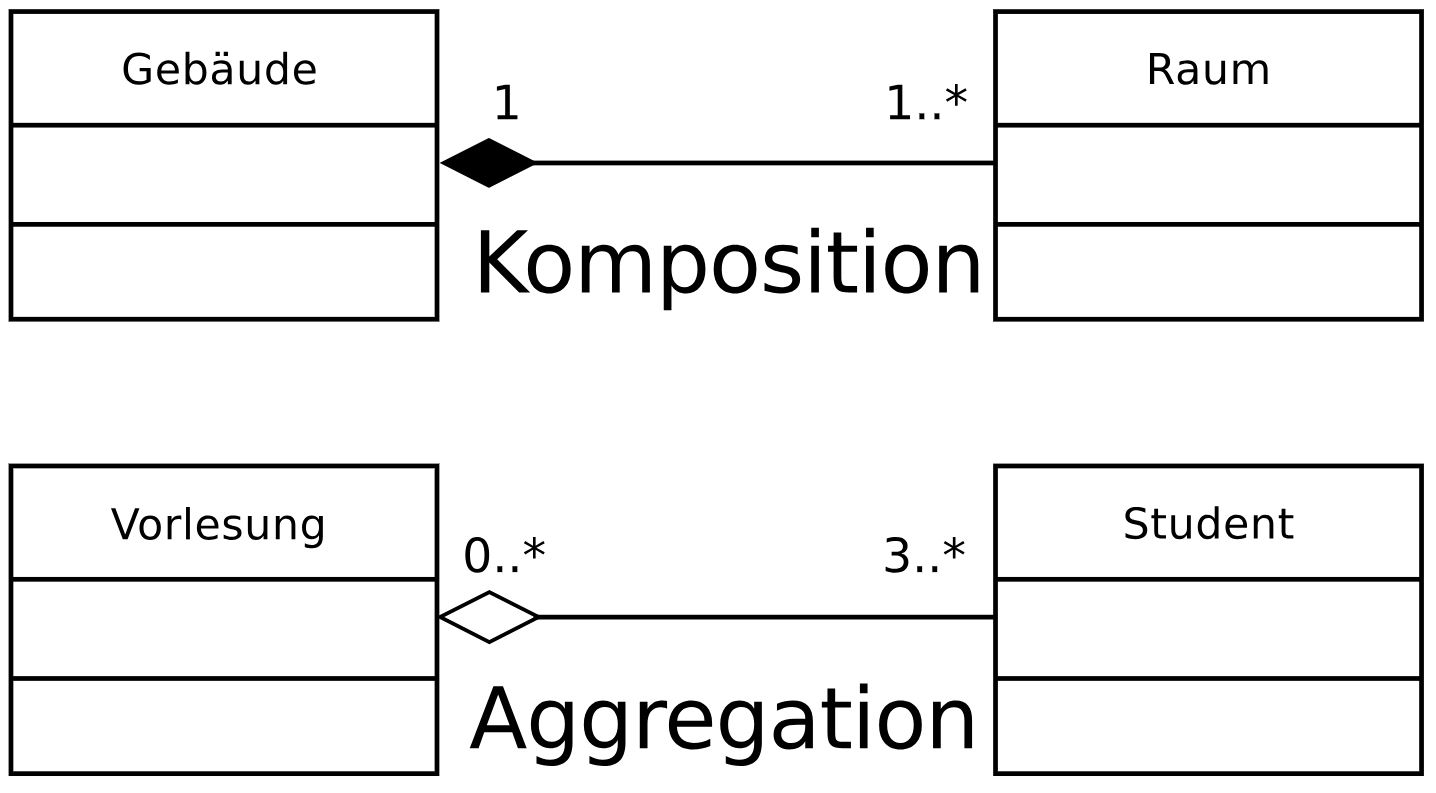
\includegraphics[width=8cm]{img/aggregation_komposition.JPG}
			\captionsetup{format=hang}
			\caption[Aggregation und Komposition]{\label{fig:aggreagtion_komposition}Aggregation und Komposition}
		\end{figure}
		
		Um nun den Reservierungsprozess im Backend abbilden zu können, werden die in Abschnitt \ref{chapter:er-diagramm} ermittelten Entitäten (\texttt{Reservierung, Ticket, Benutzer}) jeweils als eine eigene Klasse implementiert. Da in der Beziehung zwischen Benutzer und Reservierung die Reservierung einfach beteiligt ist, ist der Benutzer Teil von einer Reservierung. Dies wird durch eine Assoziation abgebildet. Ähnlich verhält sich dies in der Beziehung zwischen Ticket und Reservierung. Hier ist die Reservierung einfach beteiligt, weshalb eine Reservierung Teil von einem Ticket ist. Dieser Ausschnitt aus dem Klassendiagramm ist wie folgt grafisch nach UML-Notation abzubilden (Abbildung \ref{fig:reservation_process}):
		
		\begin{figure}[H]
			\centering 
			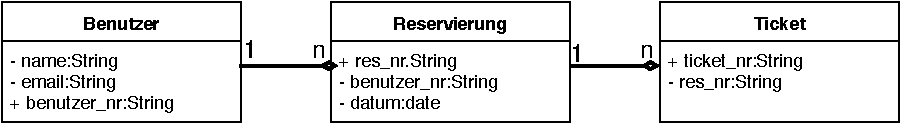
\includegraphics[width=15cm]{img/reservation_process.pdf}
			\captionsetup{format=hang}
			\caption[Klassendiagramm für den Reservierungsprozess]{\label{fig:reservation_process}Klassendiagramm für den Reservierungsprozess}
		\end{figure}
		
		Nach diesem Vorgehen wurde das komplette Klassendiagramm für das \ac{ICS} erstellt, jedoch ist wichtig anzumerken, dass ein erster Entwurf nicht die endgültige Lösung darstellt und während des Entwicklungsprozesses weitere Änderungen im Vergleich zum ER-Diagramm vorgenommen wurden. Aus diesem Grund wird in Abbildung \ref{fig:Klassendiagramm} ein automatisch generiertes Klassendiagramm gezeigt, welches den aktuellsten Stand der Anwendung repräsentiert.
		
		\begin{figure}[H]
			\centering 
			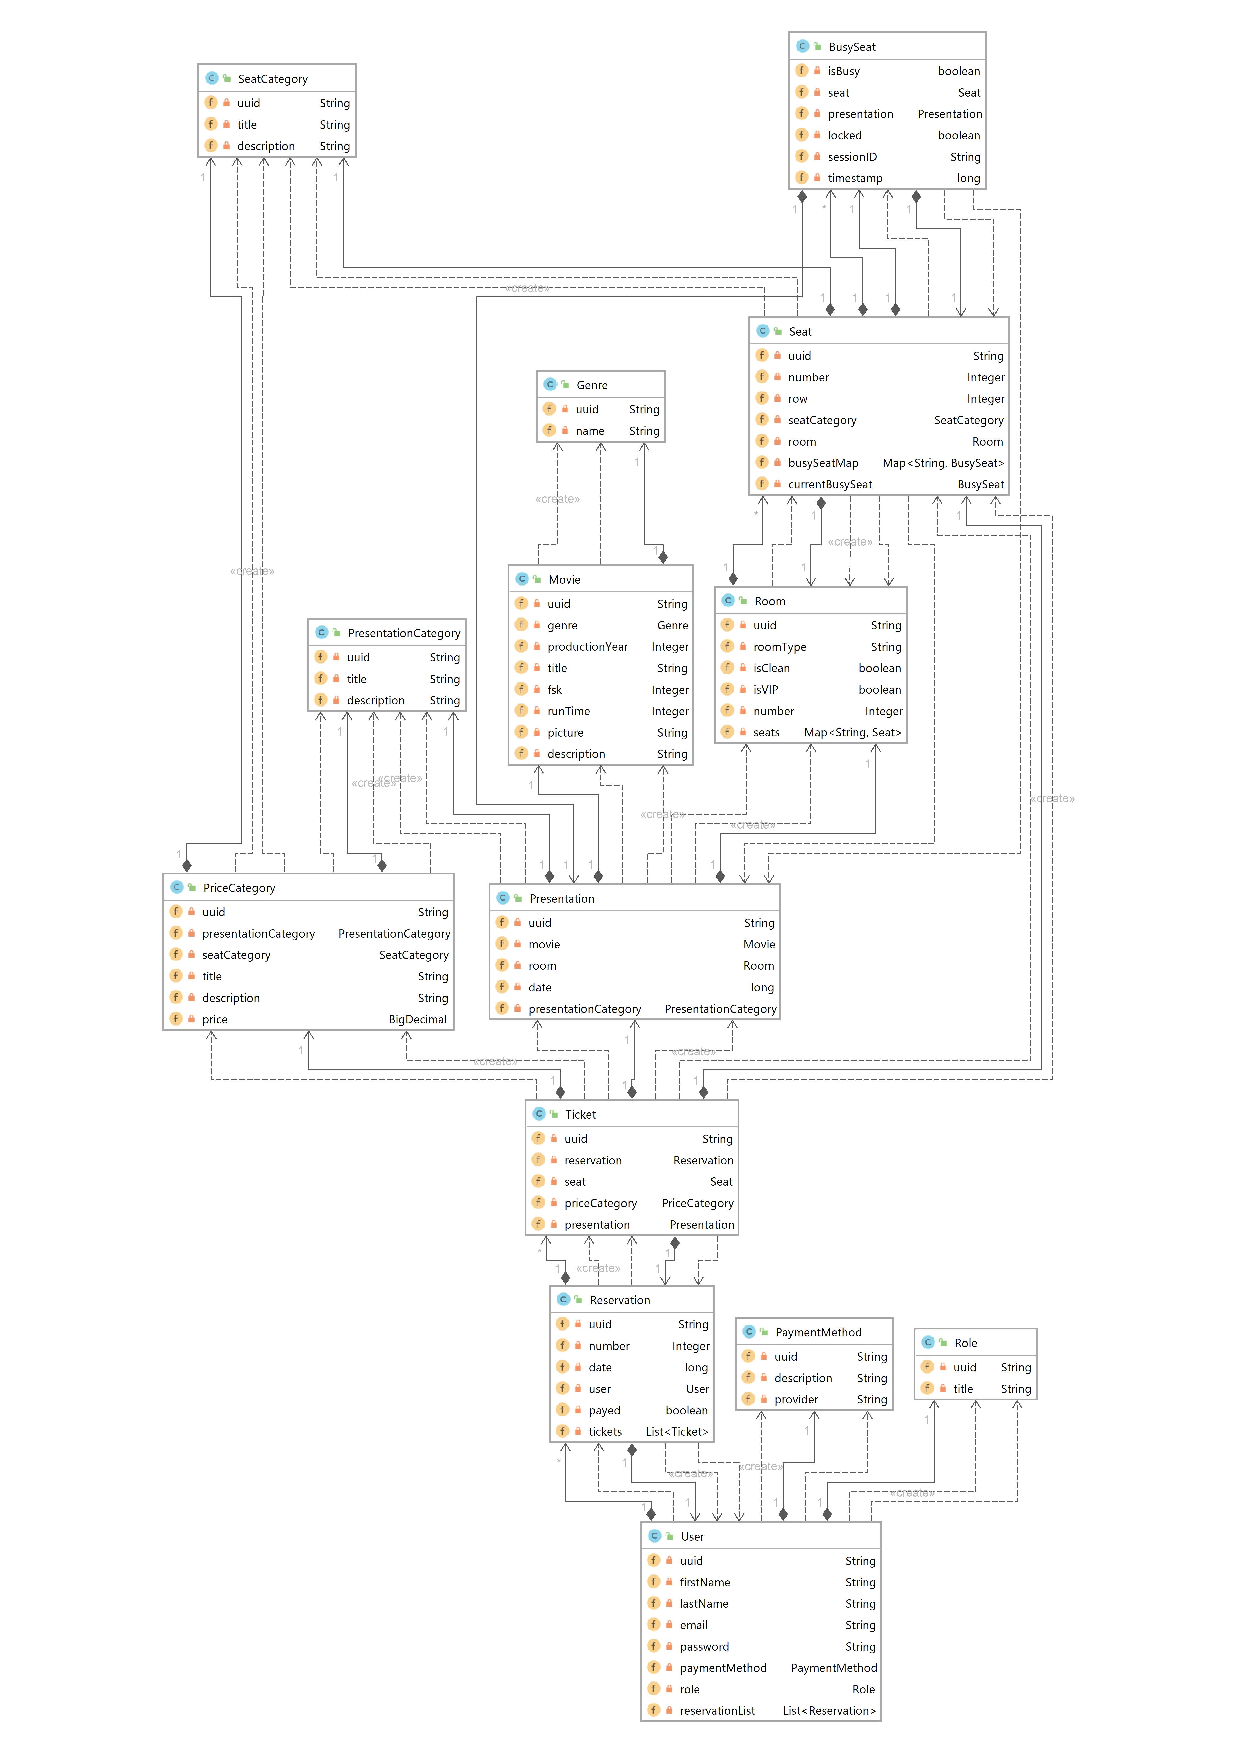
\includegraphics[width=15cm]{img/class_diagramm.pdf}
			\captionsetup{format=hang}
			\caption[Klassendiagramm]{\label{fig:Klassendiagramm}Klassendiagramm}
		\end{figure}
			
		\subsection{Dynamische Modelle}
		Als dynamisches Modell wurde ein Aktivitätsdiagramm gewählt. Dieses veranschaulicht die Abläufe in einem System und beruht auf einem Use-Case des Systems. Ein Aktivitätsdiagramm beinhaltet verschiedene \enquote{Knoten}, die einen elementaren Vorgang im System darstellen. Sie werden auch Aktionen genannt, die zu Aktivitäten zusammengefasst werden können. Um die Knoten zu verbinden und in eine Reihenfolge zu bringen, werden \enquote{Kanten} verwendet. Diese werden mittels Pfeilen dargestellt, wodurch die Reihenfolge vorgegeben wird. 
				
		Beginn und Ende einer Aktivität werden mithilfe eines ausgefüllten Punktes dargestellt, wobei der Endpunkt der Aktivität von einem Kreis umgeben ist. Verzweigungen können in einem Aktivitätsdiagramm mittels \enquote{Rauten} dargestellt werden. Dabei wird textuell hinzugefügt, um welche Entscheidung es sich handelt. 
				
		Abbildung \vref{fig:aktivitätReservierung} veranschaulicht die Aktionen, die ein Benutzer durchläuft, um Karten reservieren zu können. Er startet mit dem Ansehen der Startseite und endet mit einer erfolgreichen Reservierung. Dabei kann der Benutzer zunächst auf der Startseite nach einem passenden Film suchen. Wenn dort kein passender Film vorhanden ist, kann der Nutzer in die Programmübersicht wechseln. Sollte dort ebenfalls kein passender Film vorhanden sein, endet die Aktivität an dieser Stelle. 
								
		Falls jedoch ein passender Film auf Startseite oder Programmübersicht vorhanden ist, besteht die nächste Aktion aus dem Anklicken des Films. Nachfolgend wählt der Benutzer eine Vorstellung und die gewünschten Sitze aus. Die Reservierung wird im Hintergrund ausgeführt, wodurch das Sperren der ausgewählten Sitze vorgenommen wird, falls diese noch nicht gesperrt sind. Für den Fall, dass die Sitze bereits durch einen anderen Nutzer gesperrt sind, wird der Benutzer zur Auswahl von Sitzen zurückgeführt. 
								
		Wenn die Sitze noch frei sind, können diese durch die Eingabe der Benutzerdaten, bei Reservierung als Gast, reserviert werden. Das System prüft die Vollständigkeit der Angaben. Bei Unvollständigkeit wird der Nutzer wieder zurück zu der Auswahl der Sitze geführt. Andernfalls wird die Reservierung bestätigt und der Benutzer kann die Bestätigung einsehen. Damit ist der Reservierungsvorgang abgeschlossen und die Aktivität endet.   
						 
		Informationen zu den Aktionen, die in Frontend und Backend vorgenommen werden, um die Aktion eines Benutzers umzusetzen, können dem Anhang \vref{fig:adResAusführlich} entnommen werden.
				
		\begin{figure}[H]
			\centering 
			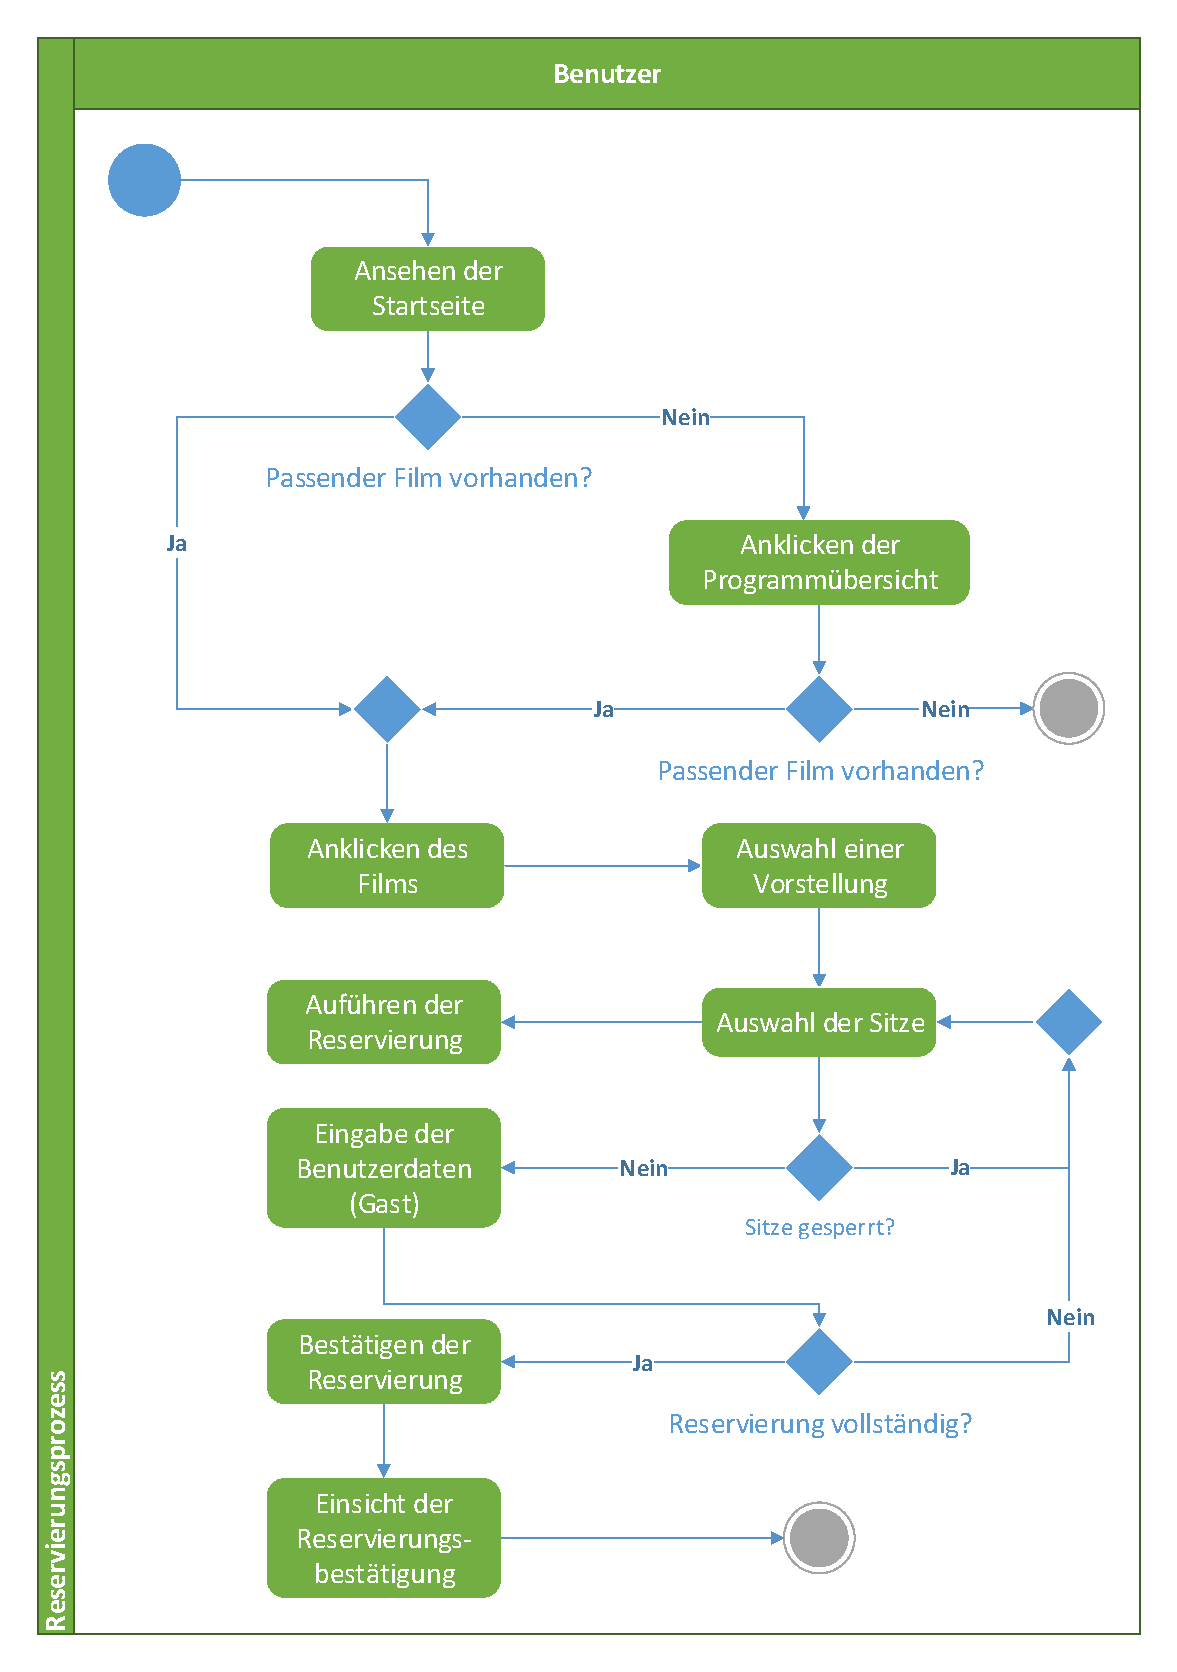
\includegraphics[width=12cm]{img/adReservierung_min.pdf}
			\captionsetup{format=hang}
			\caption[Aktivitätsdiagramm Reservierung]{\label{fig:aktivitätReservierung} Aktivitätsdiagramm Reservierungsvorgang}
		\end{figure}
				
			